%//cSpell:disable
% LTeX: enabled=false
\documentclass[a4paper,ngerman, headheight=28pt,12pt, footheight=27pt]{scrartcl}



% PACKAGES
\usepackage[a4paper,left=3cm,right=4cm,top=2.5cm,bottom=2.5cm]{geometry}

\usepackage{fontspec}
\usepackage{hyphenat}
\usepackage{babel}


% Für Code
\usepackage[outputdir=build]{minted}
\usepackage{csquotes}

% Svg Image with Inkscape
\usepackage{svg}
\usepackage{relsize}
\usepackage{setspace}

\usepackage{lineno}

\usepackage{tabularray}
\usepackage{float}

% Appendix
\usepackage{appendix}

% Title Spacing

\RedeclareSectionCommand[
  %runin=false,
  afterindent=false,
  beforeskip=.5\baselineskip,
  afterskip=.25\baselineskip]{section}
\RedeclareSectionCommand[
  %runin=false,
  afterindent=false,
  beforeskip=.25\baselineskip,
  afterskip=.125\baselineskip]{subsection}
\RedeclareSectionCommand[
  %runin=false,
  afterindent=false,
  beforeskip=.175\baselineskip,
  afterskip=.0625\baselineskip]{subsubsection}


% Literaturverzeichnis
\usepackage[
backend=biber,
style=alphabetic,
sorting=nty,
maxbibnames=99
]{biblatex}

\addbibresource{refs_facharbeit.bib}

\DeclareLabelalphaTemplate{
  \labelelement{
    \field[final]{shorthand}
    \field{label}
    \field[strwidth=2,strside=left,ifnames=1]{labelname}
    \field[strwidth=1,strside=left]{labelname}
  }
  \labelelement{
    \field[strwidth=2,strside=right]{year}
  }
}
%//TODO Change font back to calibri
\IfFileExists{/etc/motd}{\setmainfont{calibri}[
  Path=./fonts/,
  Extension=.ttf,
  UprightFont=*-Regular,
  BoldFont=*-Bold,
  ItalicFont=*-Italic,
  BoldItalicFont=*-BoldItalic,
]}{\setmainfont{Calibri}}

% Used for babel hypernate
\defineshorthand{~-}{\hyp{}}

\MakeOuterQuote{"}

\newcommand{\LongMinus}{–}

% LTeX: enabled=true
%//cSpell:enable
% Die nächsten vier Felder bitte anpassen:
\newcommand{\Titel}{Dezentralisierte asymmetrische \\ Verschlüsselung über Tor} % Titel für Facharbeit
\newcommand{\SubTitel}{Die Lösung für sicheres Messaging?}

\newcommand{\PageTitel}{Dezentralisierte asymmetrische Verschlüsselung \\ über Tor \LongMinus{} Die Lösung für sicheres Messaging?} % Seitentitel für Facharbeit
\newcommand{\Author}{Hendrik Lind}     % Ich
\newcommand{\Department}{Seminarfach Informatik}
\newcommand{\School}{Windthorst-Gymnasium Meppen}
\newcommand{\Country}{Deutschland}
\newcommand{\Abgabe}{20. November 2023}

\newcommand{\thesisDegree}{Facharbeit}
\newcommand{\faculty}{Seminarfach Informatik}
\newcommand{\thesisPlaceDate}{\today}

\newcommand{\vcite}[1]{\cite[vgl.][]{#1}}
\newcommand{\vebd}{[vgl. ebd.]}

% Tor Stuff
\newcommand{\entryn}{\textit{Entry Node\,}}
\newcommand{\relayn}{\textit{Relay Node\,}}
\newcommand{\relayns}{\textit{Relay Nodes\,}}
\newcommand{\exitn}{\textit{Exit Node\,}}
\newcommand{\exitns}{\textit{Exit Nodes\,}}
\newcommand{\nodes}{\textit{Nodes\,}}
\newcommand{\node}{\textit{Node\,}}
\newcommand{\onion}{\textit{Onion\,}}
\newcommand{\circuit}{\textit{Circuit\,}}
\newcommand{\circuits}{\textit{Circuits\,}}
\newcommand{\introp}{\textit{Introduction Point\,}}
\newcommand{\introps}{\textit{Introduction Points\,}}
\newcommand{\renp}{\textit{Rendezvous Point\,}}

% Implementation stuff
\newcommand{\identity}{\textit{Identity\,}}

%//cSpell:disable
% LTeX: enabled=false

% Kopf- und Fußzeilen
\usepackage{scrlayer-scrpage, lastpage}
\setkomafont{pageheadfoot}{\large\textrm}
\lohead{\PageTitel}
\rohead{\Author}
\cfoot*{\thepage{}/\pageref{LastPageDoc}}

% Position des Titels
\usepackage{titling}
\setlength{\droptitle}{-1.0cm}


% Für mathematische Befehle und Symbole
\usepackage{amsmath}
\usepackage{mathtools}
\usepackage{amssymb}
\usepackage{wrapfig}

% Für Bilder
\usepackage{graphicx}
\usepackage{graphbox}


% Für PDF
\usepackage{pdfpages}

\graphicspath{ {./img/} }


% 1.5 Line spacing
\setstretch{1.5}


% Diese beiden Pakete müssen zuletzt geladen werden
\usepackage[hidelinks]{hyperref} % Anklickbare Links im Dokument
\usepackage{cleveref}

% Titlepage required things


% Necessary packages for the titlepage:
\usepackage{tikz}
\usetikzlibrary{calc}
%\usepackage{graphicx}
% \usepackage{newtxtext}
%\usepackage{float}
\usepackage{comment}
% This command changes the font style where SLU promotes Arial
%\newenvironment{myfont}{\fontfamily{phv}\selectfont}{\par}


% Add line breaks to urls
\apptocmd{\UrlBreaks}{\do\f\do\m}{}{}
\setcounter{biburllcpenalty}{9000}% Kleinbuchstaben
\setcounter{biburlucpenalty}{9000}% Großbuchstaben

% Optionally show or hide code

\newif\ifshow % toggle true or false based on if want to hide section
\showtrue % show the sections
%\showfalse % hide the sections

\usepackage{version}
\ifshow
  \includeversion{minted}
  \includeversion{wrap}
  \includeversion{equation}
\else
  \excludeversion{minted}
  \excludeversion{wrap}
  \excludeversion{equation}
\fi



% Used to adjust small overfulls
\usepackage{microtype}


% Hyphenations
\hyphenation{an-ge-wie-sen}


% Ensure that the url is in has the main font
\usepackage{url}
\urlstyle{same}

% Facharbeit

\begin{document}
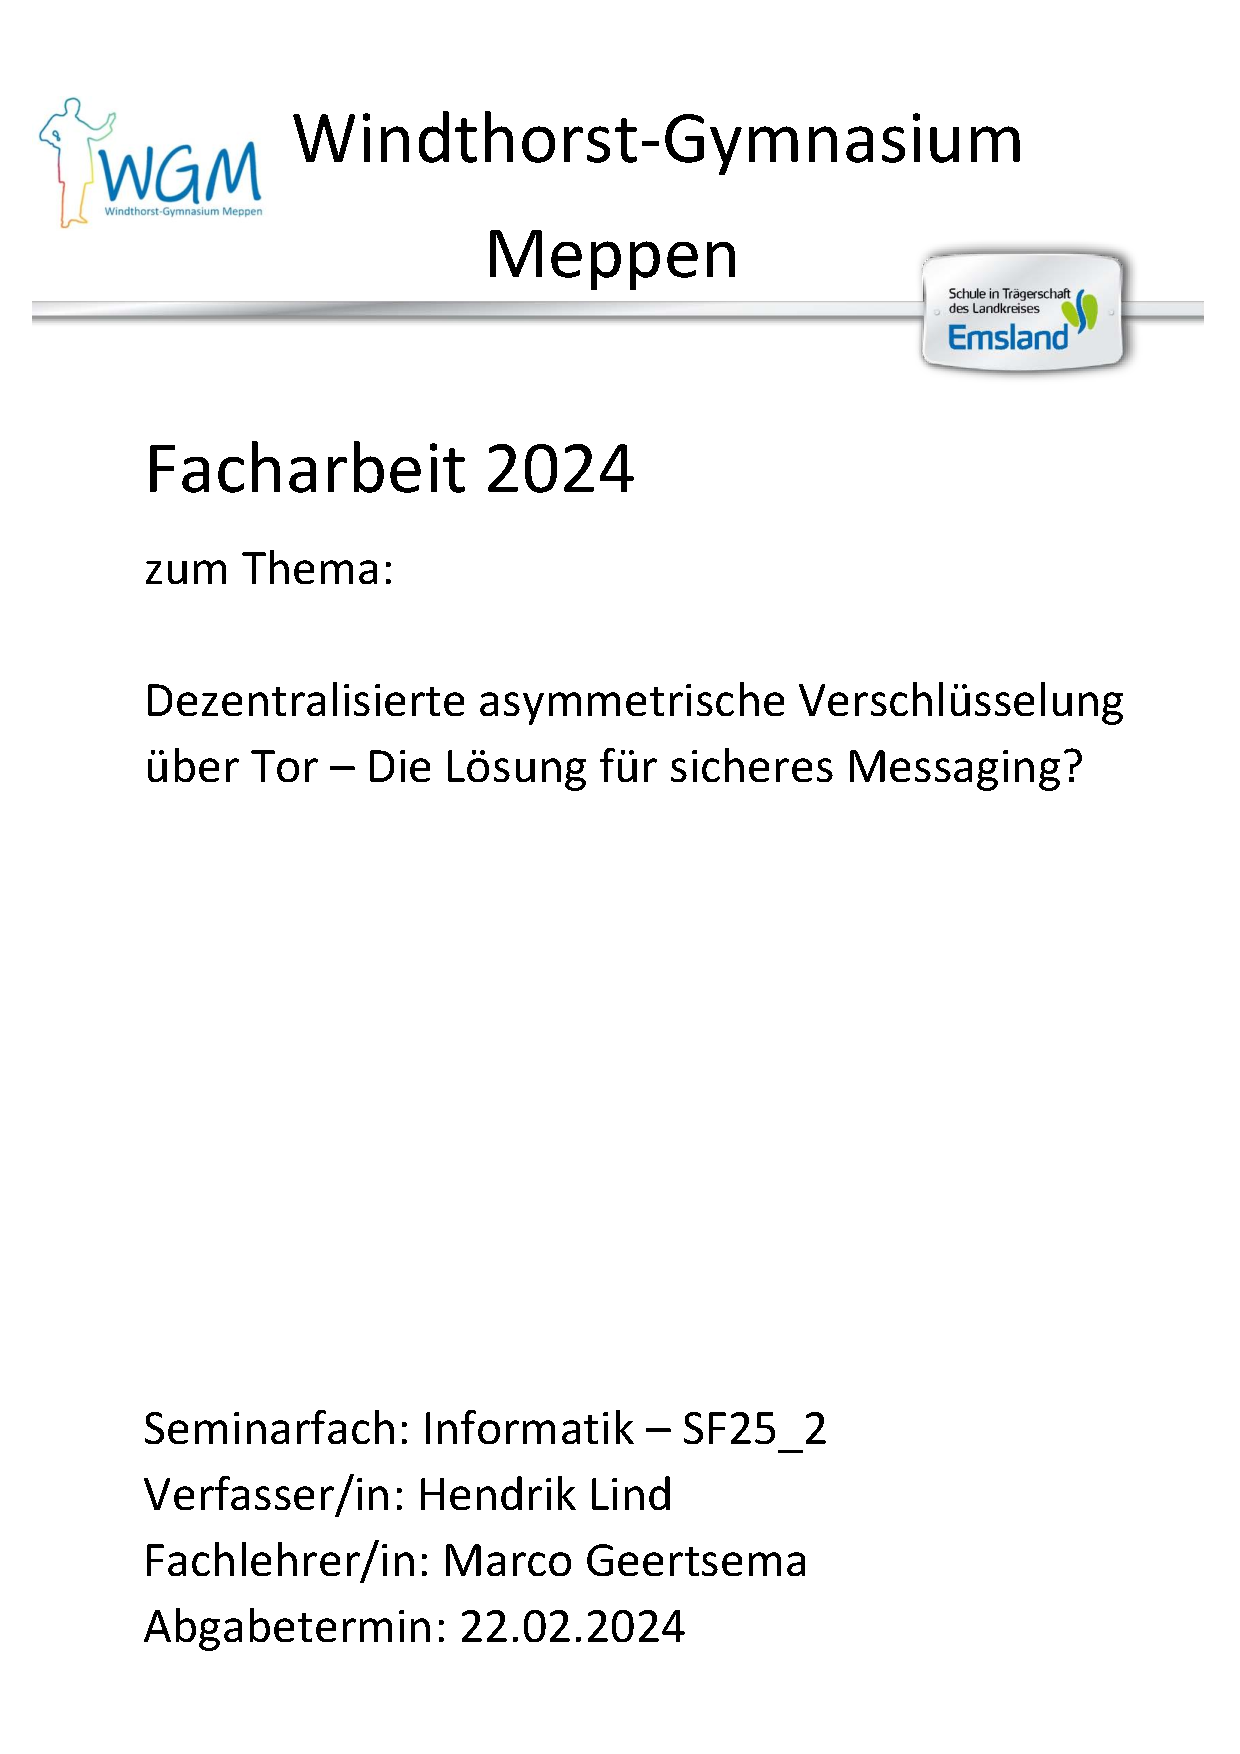
\includepdf[pages=1]{img/frontpage.pdf}
\pagestyle{empty}
\tableofcontents
\clearpage
\pagestyle{plain}
%% To add this template to the main.tex file, just add the command "% To add this template to the main.tex file, just add the command "% To add this template to the main.tex file, just add the command "\include{titlePageSLU} after "\begin{docuemnt}" in the main.tex file


% In this segment, enter the desired data to be shown at the title page
\newcommand{\thesisAuthor}{Firstname Lastname}
\newcommand{\thesisTitle}{Interesting Thesis Title}
\newcommand{\thesisSubTitle}{little bit more descriptive}
\newcommand{\thesisTitleTranslated}{Translated Headline}
\newcommand{\thesisDegree}{Master thesis project}
\newcommand{\university}{Swedish University of Argicultural Science, SLU}
\newcommand{\credits}{30 hp}
\newcommand{\faculty}{Faculty of blablabalba}
\newcommand{\thesisPlaceDate}{Place of puplication, Year}
\newcommand{\company}{Company name}

%------------------------------------------------------------------------------
\begin{titlepage}
\thispagestyle{empty}
\myfont

% Use this line of code if both SLU loggo and company/other institution loggo is desired. The positions are possible to change with the \hspace and \vspace syntax.
\begin{figure} [H]
\vspace{-3cm}
 \centering
\begin{minipage}[t]{.45\linewidth}
  \raggedright
  % Upload and include SLU loggo here:
  \hspace*{-2cm}
\includegraphics[width=\linewidth]{slu_logo_webb.png}
  
\end{minipage}%
  \begin{minipage}[t]{.45\linewidth}
  \vspace{-3.3cm}
 \raggedleft
% Upload and include other loggo here (loggo of wikipedia is used as an example):
 \hspace*{1cm}
\includegraphics[width =0.5\textwidth]{wikilogo.png} \hspace*{-1cm}
 
\end{minipage}
\end{figure}


% If only the logo for SLU is desired, delete "\begin{comment}" and "\end{comment}" to use this line of code:
\begin{comment}
\begin{figure}
\vspace{-3cm}
    \hspace*{-2cm}
\includegraphics[width = 0.3\textwidth]{slu_logo_webb.png}\hspace*{-2cm}
\end{figure}
\end{comment}


% Adds background picture. Delete code if no background picture is wanted.
\begin{tikzpicture}[overlay, remember picture]
\node[anchor=south west, 
      xshift=-0.2cm, 
      yshift=-0.2cm] 
     at (current page.south west)
     {
\includegraphics[width = 1.8\textwidth, height = 9cm]{background.png}}; 
\end{tikzpicture}


\vspace{1cm}
\par
\noindent
\Huge
\textbf{\thesisTitle}
\vspace{0.2cm}
\LARGE
\par
\noindent
- \thesisSubTitle\\
\rule[0.3cm]{\linewidth}{2pt}
\Large

% Delete this line if no translation is desired
\noindent
\textit{\thesisTitleTranslated}

\vspace{2cm}
\noindent
\LARGE
\thesisAuthor\\
\vspace{4 cm}
\small
\par \noindent
\thesisDegree $\cdot$ \credits
\par \noindent
\university
\par \noindent
\faculty
\par \noindent
\company
\par \noindent
\thesisPlaceDate

\end{titlepage}
 after "\begin{docuemnt}" in the main.tex file


% In this segment, enter the desired data to be shown at the title page
\newcommand{\thesisAuthor}{Firstname Lastname}
\newcommand{\thesisTitle}{Interesting Thesis Title}
\newcommand{\thesisSubTitle}{little bit more descriptive}
\newcommand{\thesisTitleTranslated}{Translated Headline}
\newcommand{\thesisDegree}{Master thesis project}
\newcommand{\university}{Swedish University of Argicultural Science, SLU}
\newcommand{\credits}{30 hp}
\newcommand{\faculty}{Faculty of blablabalba}
\newcommand{\thesisPlaceDate}{Place of puplication, Year}
\newcommand{\company}{Company name}

%------------------------------------------------------------------------------
\begin{titlepage}
\thispagestyle{empty}
\myfont

% Use this line of code if both SLU loggo and company/other institution loggo is desired. The positions are possible to change with the \hspace and \vspace syntax.
\begin{figure} [H]
\vspace{-3cm}
 \centering
\begin{minipage}[t]{.45\linewidth}
  \raggedright
  % Upload and include SLU loggo here:
  \hspace*{-2cm}
\includegraphics[width=\linewidth]{slu_logo_webb.png}
  
\end{minipage}%
  \begin{minipage}[t]{.45\linewidth}
  \vspace{-3.3cm}
 \raggedleft
% Upload and include other loggo here (loggo of wikipedia is used as an example):
 \hspace*{1cm}
\includegraphics[width =0.5\textwidth]{wikilogo.png} \hspace*{-1cm}
 
\end{minipage}
\end{figure}


% If only the logo for SLU is desired, delete "\begin{comment}" and "\end{comment}" to use this line of code:
\begin{comment}
\begin{figure}
\vspace{-3cm}
    \hspace*{-2cm}
\includegraphics[width = 0.3\textwidth]{slu_logo_webb.png}\hspace*{-2cm}
\end{figure}
\end{comment}


% Adds background picture. Delete code if no background picture is wanted.
\begin{tikzpicture}[overlay, remember picture]
\node[anchor=south west, 
      xshift=-0.2cm, 
      yshift=-0.2cm] 
     at (current page.south west)
     {
\includegraphics[width = 1.8\textwidth, height = 9cm]{background.png}}; 
\end{tikzpicture}


\vspace{1cm}
\par
\noindent
\Huge
\textbf{\thesisTitle}
\vspace{0.2cm}
\LARGE
\par
\noindent
- \thesisSubTitle\\
\rule[0.3cm]{\linewidth}{2pt}
\Large

% Delete this line if no translation is desired
\noindent
\textit{\thesisTitleTranslated}

\vspace{2cm}
\noindent
\LARGE
\thesisAuthor\\
\vspace{4 cm}
\small
\par \noindent
\thesisDegree $\cdot$ \credits
\par \noindent
\university
\par \noindent
\faculty
\par \noindent
\company
\par \noindent
\thesisPlaceDate

\end{titlepage}
 after "\begin{docuemnt}" in the main.tex file


%------------------------------------------------------------------------------
\begin{titlepage}
\thispagestyle{empty}
% Use this line of code if both SLU loggo and company/other institution loggo is desired. The positions are possible to change with the \hspace and \vspace syntax.
\begin{figure} [H]
\vspace{-2cm}
 \centering
\begin{minipage}[t]{.45\linewidth}
  \raggedright
  % Upload and include SLU loggo here:
  \hspace*{-2cm}
\includegraphics[width=\linewidth]{wgm.png}
  
\end{minipage}%
  \begin{minipage}[t]{.45\linewidth}
  \vspace{-3.3cm}
 \raggedleft
% Upload and include other loggo here (loggo of wikipedia is used as an example):
 \hspace*{2cm}
\includegraphics[width =0.5\textwidth]{enkrypton.png} \hspace*{-1cm}
 
\end{minipage}
\end{figure}

% Adds background picture. Delete code if no background picture is wanted.
\begin{tikzpicture}[overlay, remember picture]
\node[anchor=south west, 
      xshift=-0.2cm, 
      yshift=-0.2cm] 
     at (current page.south west)
     {
\includegraphics[width = 1.8\textwidth, height = 9cm]{background.png}}; 
\end{tikzpicture}


\vspace{1cm}
\par
\noindent
\Huge
\textbf{\Titel}
\vspace{0.2cm}
\LARGE
\par
\noindent
\SubTitel\\
\rule[0.3cm]{\linewidth}{2pt}
\Large

\vspace{2cm}
\noindent
\LARGE
\Author\\
\vspace{4 cm}
\small
\par \noindent
\thesisDegree
\par \noindent
\School
\par \noindent
\faculty
\par \noindent
\thesisPlaceDate

\end{titlepage}
\setcounter{page}{1}

%//cSpell:enable
% LTeX: enabled=true
\linenumbers{}
\modulolinenumbers[5]
\section{Einleitung}
Russland, China, Iran. In diesen totalitären Staaten herrscht eine starke Zensur \vcite{AmnReport}. Allein in diesen drei Ländern sind rund 1,7 Milliarden Menschen von der Einschränkung der Meinungsfreiheit betroffen.
Wie können Bürger aus solchen Staaten ihre Meinung verbreiten, staatliche oder nichtstaatliche Organisationen auf staatskritische Situationen und Probleme aufmerksam machen, ohne sich selbst in Gefahr zu bringen? \\
Bei herkömmlichen Messengern wie WhatsApp, Signal und Co. wird zur bi- oder multilateralen Kommunikation die Telefonnummern benötigt, um untereinander in Kontakt treten zu können. Eine mögliche Gefahr besteht darin, dass sich ein totalitärer Staat als legitimer Empfänger ausgibt, wodurch Bürger und z.B. staatskritische Journalisten ihre privaten Telefonnummern an den Staat weitergeben, der dann wiederum in der Lage ist, diese Nummern zurückzuverfolgen \vcite{LocPolice}. Genau hier liegt das Problem: oppositionelle Bürger und Reporter können nicht über gewöhnliche Messenger mit der Außenwelt kommunizieren, da der Staat ihre Nummern zurückverfolgen kann, und sie mit einer weiteren Einschränkung ihrer Meinungsfreiheit oder sogar mit ihrer Verhaftung rechnen müssen \vcite{AmnReport}. \\
Die zentrale Infrastruktur, der meisten Messengern wie WhatsApp und Signal, ermöglicht es außerdem totalitären Staaten wie China, die IP-Adressen von Servern zu blockieren und sie so für Bürger und Journalisten unzugänglich zu machen \vcite{ChinaFirewall,CentralizedWhatsapp}.
%//REVIEW - Ist verschlüsselt so okay aufgebrochen?
Vor diesem Hintergrund könnte ein dezentraler, Ende-zu-Ende-ver~-schlüsselter Messenger, der über das Tor-Netzwerk kommuniziert, eine Lösung für diese Probleme darstellen. Ziel dieser Arbeit ist es, diese Lösung auf ihre Sicherheit und Praktikabilität hin zu untersuchen und zu implementieren.\\
%//NOTE - Hier habe ich den 1. Satz nicht übernommen, hat nicht ganz den Sinn getroffen
Um ein Verständnis für die Sicherheit dieses Messengers zu erlangen, geht diese Arbeit im zweiten Kapitel auf die asymmetrische Verschlüsselung und die Ende-zu-Ende-Verschlüsselung (E2EE) ein. Hierzu werden die mathematischen Zusammenhänge näher betrachtet, um im Anschluss die Sicherheit des Verfahrens beurteilen zu können.
%//REVIEW - Habe ich so ergänzt ist okay?
Dabei wird auf die Erklärung des Padding-Verfahrens der asymmetrischen Verschlüsselung verzichtet, da eine Erläuterung den Rahmen dieser Facharbeit überschreiten würde. Im dritten Kapitel wird untersucht, ob das Tor-Netzwerk eine mögliche Lösung für das Problem der Anonymität im Internet darstellt und inwieweit es die Nutzer schützt.
%//REVIEW - Wieder umformuliert
Aufbauend auf das vierte Kapitel, in dem mit der Definition und der Sicherheit von Dezentralisierung die Grundlagen gelegt werden, wird im darauffolgenden fünften Kapitel die Implementierung des Messengers beschrieben, woraufhin sechsten Kapitel auf die Nachteile des Messengers und deren Lösungsmöglichkeiten eingegangen wird. Die Arbeit endet mit dem siebten Kapitel, in welchem ein kurzes Fazit der erarbeiteten Ergebnisse gezogen wird.

\subsection{Motivation}
Mein Interesse an Themenkomplex erstreckt sich über mehrere Ebenen. Neben der asymmetrischen Verschlüsselung und der dahinterliegenden Mathematik, ist die Programmierung selbst und die Implementierung eines sicheren Messengers im Tor-Netzwerk eine meiner Hauptmotivationen mich mit diesem umfangreichen Thema zu beschäftigen. \\
Ich verfolge das Tor-Netzwerk und seine Struktur schon seit ein paar Jahren mit großem Interesse. Das Tor-Netzwerk wird oft mit dem Begriff des Darknets in Verbindung gebracht, was bei den meisten Menschen zu negative Assoziationen führt \vcite{BsiTorDarknet}. Die schwierige Rückverfolgung spielt eine große Rolle in der Anonymität des Tor-Netzwerkes und ist ein weiterer Aspekt, der mich an diesem Thema fasziniert \vebd.
%//REVIEW - Punkt hier komisch?
Zusätzlich steht der mathematische Erklärungsansatz der asymmetrischen Verschlüsselung für mich mitunter im Vordergrund meines Interesses: "Wie schafft es der Angreifer, eine verschlüsselte Nachricht nur mit dem öffentlichen Schlüssel nicht zu entschlüsseln?".
Die vielen Facetten des Tor-Netzwerks mit der Ende-zu-Ende-Verschlüsselung und der Dezentralisierung zu verbinden, sodass am Ende ein funktionierender Messenger entsteht, ist eine weitere Herausforderung, für die ich mich begeistern kann.

\subsection{Relevanz}
Durch die steigende Anzahl von Cyberangriffen geraten  Messenger immer mehr in den Fokus von Angreifern, da durch die Kompromittierung eines Messagingdienstes viele persönliche Daten erlangt werden können \vcite{Cyberattacks}. China betreibt eine ausgefeilte Analyse und Überwachung des Netzes, wodurch die eine Anonymität und Sicherheit von Messengern umso wichtiger ist \vcite{GreatFirewallChina}. Mit solch einem Messenger könnten oppositionelle Meinungen und Ansichten das autoritär geführte Land verlassen und in der Außenwelt Gehör finden. Und auch hier stellt sich wieder die Frage: "Schützt ein solcher Messenger Bürger und Journalisten in einem totalitären Staat vor möglichen Konsequenzen?".

\subsection{Methodisches Vorgehen}
Zunächst werde ich die Grundlagen der asymmetrischen Verschlüsselung, des Tor-Netzwerks und der Dezentralisierung erläutern, um dann jeweils die Sicherheit des Verfahrens zu überprüfen. Den theoretischen Hintergrund werde ich anschließend anwenden und somit einen Messenger programmieren, auf dessen Nachteile und mögliche Lösungsmöglichkeiten hinweisen, und abschließend ein Fazit ziehen.

%//REVIEW - E2EE-Method kann auch duch \vebd ersetzt werden
\section{Asymmetrische Verschlüsselung}
Um einen sicheren Nachrichtenaustausch zu gewährleisten, wird in dieser Arbeit E2EE implementiert. Bei E2EE wird die Nachricht vom Sender verschlüsselt, bevor sie an den Empfänger gesendet wird \vcite{E2EE}. Zwischengeschaltete Akteure wie Server oder mögliche Angreifer können die Nachricht somit nicht lesen \vebd. \textbf{Nur} der Empfänger oder Sender der Nachricht kann diese entschlüsseln \vcite{E2EE-Method}. Als Verfahren zur Ver- und Entschlüsselung der Nachrichten wird (unter anderem) die asymmetrische Verschlüsselung verwendet \vebd. Diese Arbeit beschränkt sich bei der asymmetrischen Verschlüsselung auf das RSA-Verfahren.

\subsection{Grundlagen}
Grundsätzlich wird bei der asymmetrischen Verschlüsselung ein Schlüsselpaar (key pair) verwendet, das aus einem privaten Schlüssel (private key) und einem öffentlichen Schlüssel (public key) besteht \vcite{Rsa-Basics}. Diese beiden Schlüssel sind mathematisch so miteinander verknüpft, dass der öffentliche Schlüssel Nachrichten \textbf{nur} verschlüsseln, aber nicht entschlüsseln kann \vebd. \textbf{Nur} der zum Schlüsselpaar gehörende private Schlüssel kann die verschlüsselte Nachricht wieder entschlüsseln (siehe \cref{fig:E2EE}) \vebd.
\begin{figure}[H]
  \centering
  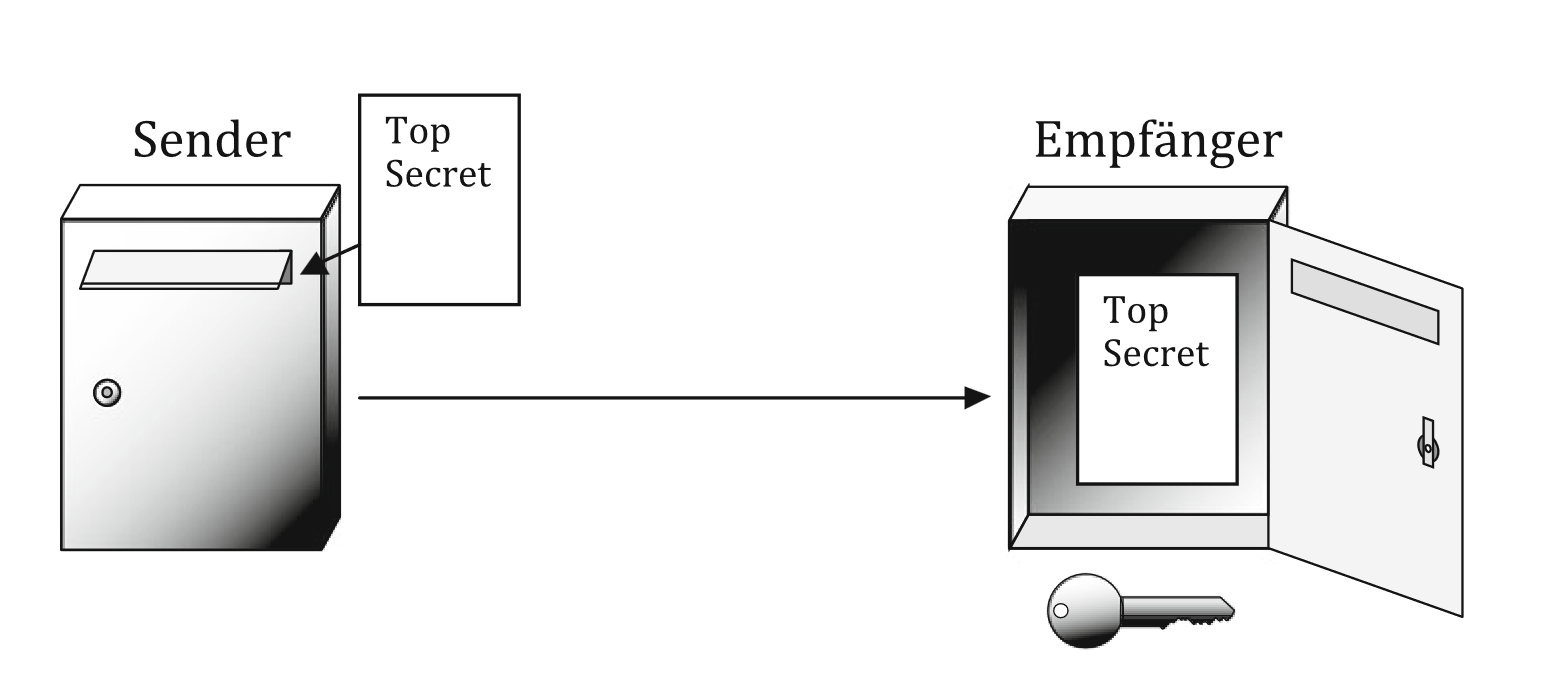
\includegraphics[width=0.75\textwidth]{Briefkasten-asymm.png}
  \caption{Jeder Sender kann mit dem öffentlichen Schlüssel die Nachricht "verschlüsseln" (also eine Nachricht in den Briefkasten werfen), aber nur der Empfänger kann den Briefkasten mit seinem privaten Schlüssel öffnen und somit die Nachricht herausnehmen \vcite{fig:Rsa-Cryptography} \label{fig:E2EE}}
\end{figure}

\subsection{Mathematische Betrachtung}
%//REVIEW - Removed newline here
Alle Variablen der folgenden Berechnungen liegen im Bereich $\mathbb{N}$ \vcite{RsaGenCond}. Zur Erzeugung des Schlüsselpaares benötigen wir zunächst zwei große zufällige Primzahlen $P$ und $Q$ \vebd. Daraus ergibt sich $n = P \cdot Q$, wobei $P \neq Q$ ist, sodass $P$ bzw. $Q$ nicht durch $\sqrt{n}$ bestimmt werden können \vebd. Der private Schlüssel setzt sich hierbei aus den Komponenten $\{ n, d \}$ zusammen, während der öffentliche Schlüssel aus $\{ n, e \}$ besteht \vcite{RsaVariables}.
\subsubsection{Eulersche Phi-Funktion}
Die eulersche Phi-Funktion spielt eine wichtige Rolle im RSA-Verfahren \vcite{TotientFuncMultiplicative}. Grundsätzlich gibt $\phi(x)$ an, wie viele positive teilerfremde Zahlen es bis $x$ gibt (für wie viele Zahlen der größte gemeinsame Teiler ($\gcd$) mit $x$ $1$ ist) \vcite{EulersTotientFunction}. So ergibt sich $\phi(6) = 2$ oder im Falle einer Primzahl $\phi(7) = 7 - 1 = 6$, also $\phi(x) = x-1$, wenn $x$ eine Primzahl ist, da jede Zahl kleiner als $x$ teilerfremd sein muss \vcite{TotientFuncMultiplicative}. Somit gilt:
\begin{equation*}
  \begin{aligned}
    \phi(n) & = \phi(P \cdot Q)                                                \\
    \phi(n) & = \phi(P) \cdot \phi(Q)                                          \\
    \phi(P) & = P -1                                          & \phi(Q) = Q -1 \\
    \phi(n) & = \left(P - 1 \right) \cdot \left( Q - 1\right)
  \end{aligned}
\end{equation*}

\subsubsection{Generierung des Schlüsselpaares}
Wie bereits erwähnt besteht sowohl der private als auch der öffentliche Schlüssel bestehen unter anderem aus der Komponente  $n$: $n = P \cdot Q$ \vcite{RsaMaths1}. Um mit dem öffentlichen Schlüssel eine Verschlüsselung durchführen zu können wir die Komponente $e$ benötigt \vebd. $e$ ist eine Zufallszahl, für welche folgende Bedingungen erfüllt sein müssen \vebd:
\begin{equation*}
  e = \begin{cases}
    1 < e < \phi(n)      \\
    \gcd(e, \phi(n)) = 1 \\
    \text{$e$ kein Teiler von $\phi(n)$}
  \end{cases}
\end{equation*}
Nachdem die Komponente $e$ gefunden wurde, ist der öffentliche Schlüssel nun vollständig und kann an den Absender übermittelt (bzw. veröffentlicht) werden. Zur Entschlüsselung einer Nachricht ist die Komponente $d$, welche im privaten Schlüssel enthalten ist, erforderlich \vcite{RsaMaths1}:
\begin{equation*}
  \begin{aligned}
    \phi(n) & = (P-1)(Q-1)          \\
    d       & = e^{-1} \mod \phi(n)
  \end{aligned}
\end{equation*}
Das Schlüsselpaar wurde nun vollständig berechnet und die beiden Schlüssel hängen mathematisch miteinander zusammen.
\subsection{Sicherheit}
Um die Sicherheit des RSA-Verfahrens bewerten zu können, müssen wir zunächst den Ver-/Entschlüsselungsprozess betrachten.
\begin{equation*}
  \begin{aligned}
    c & = m^e \mod n & \text{Verschlüsselung zu $c$ mit $m$ als Nachricht}    \\
    m & = c^d \mod n & \text{Umkehroperation (Entschlüsslung) von $c$ zu $m$}
  \end{aligned}
\end{equation*}
Damit die verschlüsselte Nachricht $c$ wieder entschlüsselt werden kann, bräuchte ein Angreifer die Komponente $d$. Dadurch, dass $d$ nur im privaten Schlüssel enthalten ist, müsste der Angreifer also selbst $d$ berechnen, welches allerdings sehr rechenintensiv ist, da diese durch $\phi(n)$ berechnet werden müsste. Eine Primfaktorzerlegung von $n$ ist also nötig \vcite{EulersTotientFunction}. Die Verschlüsselung von $m$ nach $c$ ist eine Trapdoor-Einwegfunktion \vcite{RsaTrapdoor}. Das bedeutet, dass es zwar einfach ist, $f(x) = i$ zu berechnen (im Falle der RSA Verschlüsselung), es aber unmöglich ist, von $i$ auf den ursprünglichen Wert $x$ zu schließen, ohne eine weitere notwendige Komponente zu kennen (bei dem RSA-Verfahren wäre dies die Komponente $d$) \vebd.
\begin{figure}[H]
  \centering
  \includesvg[width=0.5\textwidth]{img/Trapdoor_permutation.svg}
  \caption{Eine Visualisierung der Trapdoor-Einwegfunktion \vcite{fig:TrapdoorPermutation} \label{fig:TrapdoorFunc}}
\end{figure}
Die ausschlaggebende Größe ist hierbei die Bitlänge des Produktes $n$. Wird die Bitlänge von $n$ erhöht, steigt der Zeitaufwand, welcher für die Primfaktorzerlegung von $n$ benötigt wird, an. Somit empfiehlt das BSI eine Schlüssellänge (Länge von $n$) von mindestens 3000 Bit, um in naher Zukunft vor Angriffen geschützt zu sein \vcite{RsaKeyLength}.
\subsection{Vergleich zur symmetrischen Verschlüsselung}
%//REVIEW - Ok so?
Der wesentliche Unterschied zur asymmetrischen Verschlüsselung besteht darin, dass bei symmetrischen Verschlüsselung derselbe Schlüssel zum Ver- und Entschlüsseln verwendet wird \vcite{GeneralSymmetricCryptography}. Im Vergleich zur asymmetrischen Verschlüsselung ist die symmetrische Verschlüsselung schneller und hat keine Beschränkung der Chiffretextlänge \vcite{RsaAESAnalysis, OpensslRsaMaxLength}. Allerdings muss der Schlüssel der symmetrischen Verschlüsselung dem anderen Kommunikationspartner sicher übermittelt werden, um die Nachrichten entschlüsseln zu können \vebd.
%//REVIEW - Bisschen scuffed tbh
Die symmetrische Verschlüsselung eignet sich daher für die Verschlüsselung von Benutzerdaten des Messengers (wie z.B. Chatverläufe) mit einem benutzerdefinierten Passwort.

\section{Das Tor-Netzwerk}
Ein weiterer zentraler Aspekt dieser Arbeit ist die Anonymität der Nutzer, wobei das Tor-Netzwerk eine mögliche Lösung bietet. Das normale Routing, wie wir es täglich nutzen, eignet sich für eine hohe Anonymität nicht, da Clients direkt mit den Zielservern kommunizieren, der Zielserver somit die IP-Adresse des Clients sehen kann, wodurch eine Rückverfolgung der IP-Adresse möglich ist \vcite{TCP_IP,LocPolice}.
Genau an diesem Punkt setzt das Tor-Netzwerk an.
Um das Problem der Rückverfolgung zu lösen, besteht das Tor-Netzwerk aus vielen "\nodes" (Server des Tor-Netzwerkes), welche eingehende Tor-Verbindungen annehmen und weiterverarbeiten  \vcite{TorStructure}.
Damit ein Client eine Anfrage über das Tor-Netzwerk senden kann, sucht er sich zunächst einen "Weg", genannt \circuit, durch welchen die Anfrage des Clients geschickt werden kann \vcite{TorCircuits}.
Der \circuit, welcher für zehn Minuten gültig ist, besteht in der Regel aus drei \nodes \vebd. Nachdem der \circuit ausgelaufen ist, wird dieser durch den Client erneuert \vcite{FAQCircuitLifetime}.
Die drei \nodes werden hier in drei Kategorien unterteilt: Die \entryn, mit der sich der Client verbindet, die \relayn, welche zwischen \entryn und \exitn liegt, und die \exitn, welche sich mit dem Zielserver verbindet \vcite{TorStructure}. Der Client verschlüsselt die eigentliche Anfrage, welche er über das Tor-Netzwerk senden möchte, mehrfach, verpackt sie also in mehrere "Schalen", die eine \onion bilden, und leitet diese über den \circuit an den Zielserver weiter \vcite{TorFirstPub}.
Zunächst wird die \onion vom Tor-Client an die \entryn gesendet \vcite{TorStructure}. An jeder \node, wie der \entryn, wird eine Schale der \onion "abgeschält" (die \onion also einmal entschlüsselt), wodurch diese \node Informationen über die nächste \node der \onion erhält \vcite{TorFirstPub}. Die \node leitet nun die \onion an den nächsten Knotenpunkt weiter \vebd. Sobald \onion die \exitn erreicht hat, entfernt diese die letzte "Schale" der Anfrage, wodurch diese nun vollständig entschlüsselt ist und an den Zielserver gesendet werden kann \vebd. Dieses Routing-Verfahren ist auch als \textit{Onion-Routing} bekannt \vcite{TorStructure2}.
\begin{figure}[H]
  \centering
  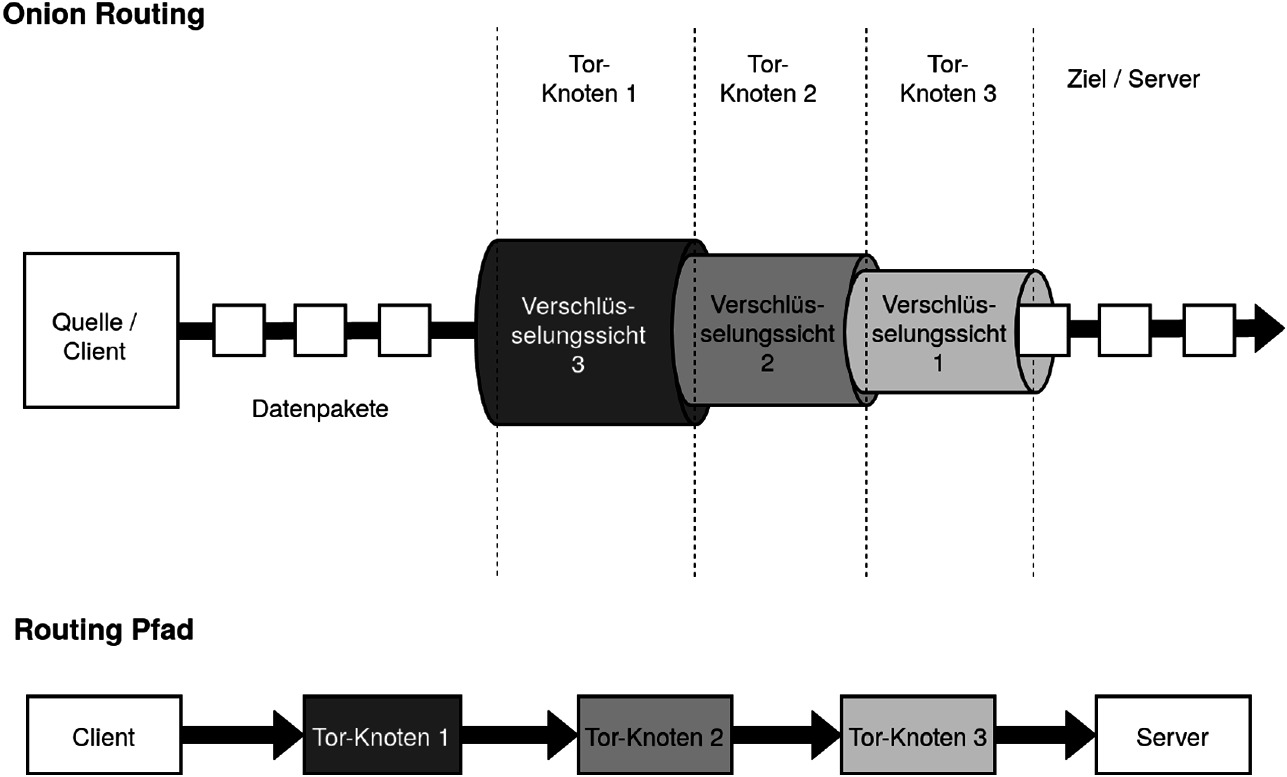
\includegraphics[width=0.65\textwidth]{TorRoutingSimple.png}
  \caption{Das Prinzip des Onion-Routings \vcite{fig:Tor-Structure} \label{fig:TorStructure}}
\end{figure}
\textbf{Nur} die \entryn kennt also die echte IP-Adresse des Clients und \textbf{nur} die \exitn weiß, an welchen Zielserver die Anfrage geschickt wurde \vcite{TorStructure}. Zwischengeschaltete \nodes wie die \relayn erkennen nur eine verschlüsselte Anfrage und haben keine Informationen über den eigentlichen Client oder Zielserver der Anfrage \vcite{EEFTor}.
Eine mögliche Schwachstelle liegt bei der \exitn, welche unverschlüsselte Anfragen an den Zielserver sendet, somit Benutzerdaten (wenn nicht mit TLS verschlüsselt) bzw. IP-Adressen ausgelesen werden können \vcite{TorBadRelay}. Durch die Einrichtung von \exitns im Tor-Netzwerk könnte ein Angreifer somit die Anonymität des Netzwerks bzw. der Benutzer gefährden (\exitn des Angreifers auch bekannt als Bad-Relay) \vebd.

\subsection{Onion Services}
Onion Services sind eine mögliche Lösung für den \exitn-Angriff \vcite{TorOnionServiceTalk}. Sie sind nicht auf \exitn angewiesen, agieren nur innerhalb des Tor-Netzwerks mit anderen \nodes und verhalten sich wie normale Tor-Clients \vebd. Onion Services sind nicht wie die Zielserver im vorherigen Beispiel über das normale Internet erreichbar, sondern nur über das Tor-Netzwerk \vcite{TorOnionService}. Im Gegensatz zu normalen öffentlichen Servern müssen bei Onion Services keine Ports geöffnet werden, damit sich ein Client mit dem Server verbinden kann, da der Onion Service mit dem Tor-Netzwerk nur über ausgehende Verbindungen kommuniziert (auch bekannt als \textit{NAT-Punching}) und alle Daten darüber geleitet werden \vebd.

\subsubsection{Verbindungsaufbau}
Zunächst erzeugt der Onion Service ein Schlüsselpaar, bestehend aus einem öffentlichen und einem privaten Schlüssel \vcite{GeeksOnionService}. Unter anderem wird nun aus dem öffentlichen Schlüssel die Adresse des Onion Service generiert, die mit ".onion" endet \vebd. Ein Beispiel für eine solche Adresse ist die der Suchmaschine DuckDuckGo: \\
\textit{duckduckgogg42xjoc72x3sjasowoarfbgcmvfimaftt6twagswzczad.onion} \vcite{DuckDuckGoLink}.
Der Onion Service verbindet sich nun wie ein normaler Client mit dem Tor-Netzwerk über einen \circuit, welcher in diesem Fall mit einer \relayn anstatt einer \exitn endet \vcite{TorOnionService}.
Der Service sendet nun eine Anfrage an die letzte \node im \circuit, sodass diese zu einem \introp wird, wodurch andere Clients später den Service erreichen können \vebd. Dieser Vorgang wiederholt sich zweimal, bis der Onion Service drei verschiedene \introps auf drei verschiedenen \circuits gefunden hat \vebd. Nun wird ein \textit{Onion Service descriptor} erstellt, welcher die Adressen der \introps und notwendige Authentifizierungsschlüssel enthält \vcite{TorSpecDirectoryInf, TorSpecDerivingKeys}. Dieser wird schließlich mit dem privaten Schlüssel des Onion Services signiert und an die Directory Authority\footnote{Die Directory Authority ist ein Server, welcher Informationen über das Tor-Netzwerk speichert und verteilt, wie z.B. die \textit{Descriptor} der Onion Services \vcite{TorDirectoryAuthority}} übermittelt, um den Onion Service für andere Tor-Clients erreichbar zu machen \vebd. Übertragen auf die Arbeit hat sich nun der Onion Service von Person A mit dem Tor-Netzwerk verbunden, aber es braucht noch Person B, die sich über ihren Tor-Client mit dem Onion Service von Person A verbindet.
Damit der Client von Person B eine Verbindung eingehen kann, fordert dieser nun die Directory Authority auf, den signierten \textit{Descriptor} des Onion Services von Person A an den Client zu senden \vcite{TorStructure}.
Der Client besitzt nun die Adressen der \introps und die Signatur des \textit{Descriptor}, sodass er die Signatur mit dem öffentlichen Schlüssel der Onion-Adresse überprüfen kann \vebd. Der Client generiert nun 20 zufällige Bytes (Secret) und sendet diese an eine zufällig ausgewählte \relayn, die nun als \renp dient \vcite{TorSpecRendezvous}. Der Client sendet das Secret auch an einen der \introps, damit der Onion Service mit dem gleichen Secret eine Verbindung zum \renp aufbauen kann \vcite{TorSpecIntroP}. Wenn der Client und der Onion Service über ihre \circuits verbunden sind, leitet der \renp die Nachrichten zwischen den beiden weiter \vcite{TorSpecRendezvous}. Der Client und der Onion Service sind somit über das Tor-Netzwerk miteinander verbunden und benötigen keine \exitns mehr, um kommunizieren zu können.

\subsection{Sicherheit}
%//TODO Nochmal Studio durchlesen, ist noch nicht schlüssig
%//TODO Angriff wurde schon von Tor gefixt, benutze OnionServiceFingerprinting
Onion Services bieten eine mögliche Lösung für die \exitn-Angriffe, da diese nur innerhalb des Tor-Netzwerkes agieren, somit nicht auf \exitns angewie~-sen sind.
Eine Deanonymisierung eines Onion Services wäre theoretisch möglich, wenn der ISP (Internet Service Provider, also z.B. Telekom, EWE, etc.) eingehende und ausgehende Verbindungen zwischen Client und Onion Service bzw. zu deren \relayn aufzeichnet und mithilfe von Machine Learning analysiert \vcite{OnionServiceFingerprinting}. Die Umsetzung der theoretischen Grundlagen war bisher unter idealisierten Bedingungen erfolgreich, jedoch sind weitere Untersuchungen notwendig, um die potenziellen Gefahren dieses Algorithmus einordnen zu können \vebd. Bei einer Zusammenarbeit der Regierungen Deutschlands, der USA und Frankreichs könnten nach der Studie 78,34 \% der \circuits deanonymisiert werden \vebd.
%//REVIEW - z.B. und von vertauschen?
Dieses Szenario erscheint jedoch unrealistisch, da die Bürger in Deutschland, den USA und Frankreich das Recht auf freie Meinungsäußerung haben und die Staaten daher höchstwahrscheinlich keine Deanonymisierungsangriffe starten werden, um die Privatsphäre von z.B. Whistleblowern zu schützen \vcite{AmnReport,ROG-USA}.
%//REVIEW - Scuffter Satz
Da über 6.500 verschiedene \nodes Teil des Tor-Netzwerkes sind, ist es in der Praxis kaum möglich alle \nodes zu blockieren, um das Netzwerk unzugänglich zu machen \footnote{Es ist zwar möglich die IP-Adressen jeglicher \relayns zu blockieren, jedoch ist dies durch Pluggable Transports umgänglich \vcite{PluggableTransports}} \vcite{DeanonymizingTorBook}.
Im Gegenzug führt die hohe Anonymität, die durch die vielen \nodes und die mehrfache Verschlüsselung erreicht wird, auch dazu, dass das Tor-Netzwerk im Vergleich zum normalen Routing fast um das 120-fache langsamer ist \vcite{TorPerformance}.

%//NOTE - Bis hier hin korrigiert
\section{Dezentralisierung}
Mit den vorgeschlagenen Konzepten ist der Messenger imstande anonym (durch das Tor-Netzwerk und Onion Services) und sicher (durch die E2EE) zu kommunizieren, jedoch wurde die Infrastruktur des Messengers noch nicht behandelt. Dafür ist die Betrachtung und Abwägung eines zentrales bzw. dezentrales Netzwerkes notwendig. \\
Ein zentrales Netzwerk, zum Beispiel das Netzwerk von WhatsApp oder Signal, besteht aus einem Hauptserver, welcher alle Anfragen der Clients weiterverarbeitet \vcite{WhatsappCentralized,SignalCentralized, CentralizedDefinition}.
%//REVIEW - Dass der Client vertrauen muss ist angegeben, aber nicht dass er es nicht überprüfen kann
Der Client muss bei dieser Netzwerkstruktur dem Hauptserver "vertrauen" und kann nicht überprüfen, ob der kompromittiert wurde \vcite{MessagingNetwork}. Dezentrale Netzwerke bestehen hingegen aus mehreren Servern, auf welche Rechenoperationen und oder Daten aufgeteilt werden \vcite{DecentralizedDefinition}.


\subsection{Sicherheit}
Durch die Abhängigkeit des zentralen Netzwerks von einem Hauptserver kann ein Angreifer gezielter, z.B. durch DDoS-Angriffe oder Kompromittierung, das gesamte Netzwerk außer Betrieb setzen oder möglicherweise Nutzerdaten (z.B. Telefonnummern bei Messengern) auslesen \vcite{CentralizedAttacks}.
Ein dezentrales Netzwerk mit einer Peer-to-Peer-Architektur\footnote{Peer-to-Peer bedeutet, dass jeder Knoten im Netzwerk sowohl Client als auch Server sein kann, die bidirektional kommunizieren \vcite{PeerToPeerDef}} bietet dagegen eine größere Angriffsfläche, sodass mehrere Knoten im Netzwerk kompromittiert oder abgeschaltet werden müssen, um das Netzwerk für deren Benutzer unzugänglich zu machen \vcite{GeeksCentralizeDecentralized}.
Es ist jedoch wichtig, dass die Knoten im Netzwerk vertrauenswürdig sind (im Beispiel des Messengers, dass nur die Gesprächsteilnehmer Teil des Netzwerks sind), um zu verhindern, dass ein Angreifer die Onion-Adressen der Gesprächsteilnehmer durch einfaches Beitreten zum Netzwerk auslesen kann.

\section{Umsetzung des Messengers}
Folgende Kriterien müssen erfüllt sein, um den Messenger sicher, anonym und einfach zu gestalten:
\begin{description}
  \item[Einfache Handhabung und Installation] \LongMinus Für die Installation und Nutzung des Messengers sollten möglichst wenig technische Kenntnisse nötig sein
  \item[Peer-to-Peer-Verbindung] \LongMinus Die Kommunikation zwischen Messengern sollte nur über eine direkte Verbindung erfolgen
  \item[Anonymität] \LongMinus Verbindungen zwischen Messengern nur das Tor-Netzwerk, keine Anfragen über das normale Internet
  \item[Sicherheit] \LongMinus Verschlüsselte Speicherung von Chatverläufen und Schlüsselpaaren, um Auslesen der Daten (z.B. durch totalitäre Staaten) zu verhindern
  \item[E2EE] \LongMinus Verschlüsselung der Nachrichten und Verifikation des Kommunikationspartners
\end{description}
Damit der Benutzer keine Konsole verwenden muss, um den Messenger zu benutzen, habe ich eine Desktopanwendung mit Rust und Tauri entwickelt. Tauri erfordert hierbei keine zusätzlichen Interpreter oder Bibliotheken, was die Installation vereinfacht.
Außerdem kann die Anwendung für Windows, Linux und macOS kompiliert werden \vcite{RustCompile}. Rust bietet eine hohe Performance und ist Memory Safe, wodurch viele Sicherheitslücken, wie Buffer Overflows, verhindert werden können \vcite{RustSecurity}. Das Tauri Framework bietet hier zwischen dem User Interface (UI), welches ich in Typescript und React programmiert habe, und dem Rust-Backend eine Schnittstelle, um Daten (\textit{payloads}) zwischen Frontend und Backend zu versenden \vcite{TauriPayloads}. Ich werde in diesem Kapitel nicht auf die Implementierung des Frontends eingehen, da dieser nur für die Benutzeroberfläche zuständig ist und keine weiteren Funktionalitäten bietet.

\subsection{Peer-to-Peer-Verbindung}
Wichtig bei der Peer-to-Peer-Funktionalität ist, dass der Messenger sowohl ein Client als auch ein Server sein kann, um Nachrichten zu empfangen und zu senden.
Um als Server zu agieren, startet jeder Messenger einen HTTP-Server, der einen HTTP-Endpunkt anbietet (in diesem Messenger \textit{/ws/}), mit welchem Clients eine Websocket\footnote{Ein Protokoll für bidirektionale Kommunikation zwischen Server und Client über HTTP \vcite{WebsocketDef}}-Verbindung aufbauen können. Der Server ist somit in der Lage, sowohl Packets zu empfangen als auch zu senden.
\begin{minted}[breaklines]{rust}
HttpServer::new(|| {
    return App::new()
        // Return the default message to tell other clients that this server is actually alive
        .service(hello)
        // The websocket endpoint
        .route("/ws/", web::get().to(ws_index));
})
// Bind just to localhost and run
.bind(("127.0.0.1", CONFIG.service_port()))?
.run()
.await?;
\end{minted}

Analog dazu hat jeder Messenger auch einen Websocket-Client, der sich direkt über das Tor-Netzwerk mit den anderen Messengern verbinden kann. Der Verbindungsaufbau zu anderen Messengern sieht wie folgt aus:
\begin{minted}[breaklines]{rust}
/// `onion_hostname` is the onion address of the other messenger to connect to
pub async fn new(onion_hostname: &str) -> Result<Self> {
  // [...]
  let connect_host = onion_hostname.to_string();

  //[...]

  // The address which is used to connect to the websocket
  let onion_addr = format!("ws://{}.onion/ws/", connect_host);

  debug!("[CLIENT] Creating proxy...");

  // Creating the Socks5Proxy client which is used to connect to the tor network
  let proxy = SocksProxy::new()?;
  debug!("[CLIENT] Connecting Proxy...");
  let mut onion_addr = Url::parse(&onion_addr)?;
  onion_addr
      .set_scheme("ws")
      .or(Err(anyhow!("[CLIENT] Could not set scheme")))?;

  // Connecting to the destination host using the proxyy
  let sock = proxy.connect(&onion_addr).await?;

  //[...]
  // Connecting to the websocket with the client
  let (ws_stream, _) = tokio_tungstenite::client_async(&onion_addr, sock).await?;

  // [...]
}
\end{minted}
Damit zwei Benutzer über den Messenger Nachrichten versenden können, muss ein Messenger die Rolle des Clients und der andere die Rolle des Servers übernehmen. Dadurch, dass jeder Messenger sowohl Client als auch Server sein kann, müssen empfangene Nachrichten von Client und Server zusammengeführt und an das Frontend übermittelt werden, welches in der Bibliothek \textit{messaging} implementiert ist:
\begin{minted}[breaklines]{rust}
/// A Manager which holds the connections by receiver name
pub struct MessagingManager {
  /// The connections by receiver name
  pub(crate) connections: Arc<RwLock<HashMap<String, Connection>>>,
}

/// A generalized connection struct that can be used for both the client and the server
#[derive(Debug, Clone)]
pub struct Connection {
    pub(super) info: Arc<RwLock<ConnInfo>>,
    read_thread: Arc<Option<ConnectionReadThread>>,
    pub(crate) self_verified: Arc<RwLock<bool>>,
    pub(crate) verified: Arc<RwLock<bool>>,
    pub(super) receiver_host: String,

    notifier_ready_tx: Sender<()>,
    notifier_ready_rx: Receiver<()>,
}
\end{minted}
Der \textit{MessagingManager} speichert sowohl Client-Server(C2S)- als auch Server-Client\\(S2C)-Verbindungen in einem allgemeinen Konstrukt, der \textit{Connection}. Diese \textit{Connection}s werden in einer \textit{HashMap} gespeichert. Der \textit{MessagingManager} stellt dem Frontend eine generelle Schnittstelle zum Senden und Empfangen von Nachrichten zur Verfügung.
\begin{figure}[H]
  \centering
  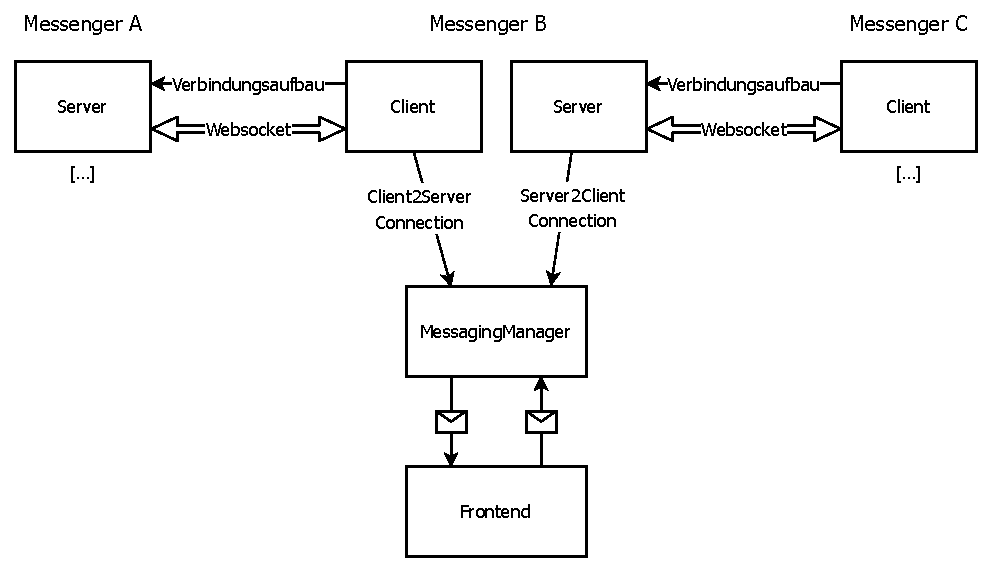
\includegraphics[width=\textwidth]{diagrams/messaging_messenger.pdf}
  \caption{Mögliches Beispiel für Messenger B, welcher eine Verbindung zu Messenger A aufgebaut hat, und Messenger C, welcher mit Messenger B verbunden ist \label{fig:MessagingMessenger}}
\end{figure}
Wenn in diesem Beispiel das Frontend von Messenger B eine Anfrage an den \textit{MessagingManager} schickt, eine Nachricht an Messenger A zu senden, wird die Nachricht verschlüsselt und an den entsprechenden Client weiterleitet. Der Client sendet nun die Nachricht über die Websocket-Verbindung an den Server von Messengers A.


\subsection{Tor-Netzwerk}
Damit der Messenger das Tor-Netzwerk verwenden kann, muss zunächst eine Verbindung zum Tor-Netzwerk hergestellt werden, welches über die \textit{tor-proxy} Bibliothek geschieht. Der HTTP-Server wird über den Tor-Proxy in das Tor-Netzwerk als Onion Service eingebunden. Damit sich der Tor-Proxy gestartet werden kann, wird eine Konfigurationsdatei benötigt, welche durch die \textit{tor-proxy} Bibliothek erstellt wird:
\begin{minted}[breaklines]{rust}
/// Converts the configuration to a `torrc` file format
async fn to_text(&self) -> Result<String> {
    let data = PathBuf::from(self.data_dir());

    let geo_ip = data.clone().join("geoip");
    let geo_ip6 = data.clone().join("geoip6");

    #[allow(unused_mut)]
    let mut config = format!(
        "SocksPort {}
HiddenServiceDir \"{}\"
HiddenServicePort 80 {}
DataDirectory \"{}\"
GeoIPFile \"{}\"
GeoIPv6File \"{}\"",
        self.get_socks_host(),
        self.service_dir().to_string_lossy().replace("\\", "/"),
        self.get_hidden_service_host(),
        self.data_dir().to_string_lossy().replace("\\", "/"),
        geo_ip.to_string_lossy().replace("\\", "/"),
        geo_ip6.to_string_lossy().replace("\\", "/"),
    );

    //[...]

    Ok(config)
}
\end{minted}
Nun muss nur noch der Tor-Proxy gestartet werden:
\begin{minted}[breaklines]{rust}
let mut child = Command::new(TOR_BINARY_PATH.clone());
child.args(["-f", &get_torrc().to_string_lossy()]);
child.current_dir(TOR_BINARY_PATH.parent().unwrap());
child.stdout(Stdio::piped());
child.stderr(Stdio::piped());
//[...]
let child = child.spawn()?;
\end{minted}
Wenn der Proxy gestartet ist, werden eingehende Verbindungen zum Onion Service dieses Messengers auf den Port des HTTP-Servers umgeleitet.
Der Messenger ist also mit dem Tor-Netzwerk verbunden und der HTTP-Server ist über eine Onion Adresse erreichbar. Andere Messenger können sich folglich anonym über das Tor-Netzwerk mit diesem Messenger verbinden.
\subsection{Sicherheit}
Ein symmetrisch verschlüsselter Datenspeicher wird durch die Bibliothek \textit{secure-storage} implementiert. Mit dieser Bibliothek können beliebige \textit{Structs} in Text umgewandelt und verschlüsseln bzw. ausgelesen und entschlüsselt werden. Die \textit{storage-internal} Bibliothek verwendet hierbei die Methoden der \textit{secure-storage} Bibliothek und dient als Wrapper, um die Daten auf der Festplatte zu speichern und wieder auszulesen. Der Datenspeicher enthält hierbei eine \textit{HashMap}, die als Schlüssel die Onion Adresse anderer Messengers und als Wert die Chatinformationen enthält. Chatinformationen sind zum Beispiel gesendete oder empfangene Nachrichten, Schlüsselpaare und öffentliche Schlüssel.
\begin{minted}[breaklines]{rust}
#[derive(Clone, Debug, Serialize, Deserialize, Zeroize, ZeroizeOnDrop)]
pub struct StorageChat {
  /// All messages sent to this receiver or received from this receiver
  pub messages: Vec<ChatMessage>,
  //[...]

  /// The public key which is used to encrypt messages when being sent to the receiver [...]
  #[zeroize(skip)]
  pub rec_pub_key: Option<PublicKey>,
  /// Private key of this messenger used to decrypt the messages that are being received [...]
  pub priv_key: PrivateKey,
}
\end{minted}
Der \textit{StorageChat} enthält dabei entweder die an den Empfänger gesendeten oder von ihm empfangenen Nachrichten (\textit{messages}), den öffentlichen Schlüssel des Kommunikationspartners (\textit{rec\_pub\_key}) und den privaten Schlüssel des Chats \textit{priv\_key}.
Um die Nutzerdaten vor weiteren möglichen Angriffen zu schützen, verwende ich die Bibliothek \textit{zeroize}, die sensible Daten (wie private Schlüssel) aus dem Arbeitsspeicher löscht, wenn die Applikation geschlossen wird (Zeroization) \vcite{Zeroization}. Zudem ist es durch die symmetrische Verschlüsselung des Datenspeichers für Angreifer nicht möglich (sofern die Applikation geschlossen ist), private Schlüssel oder Chatverläufe auszulesen, wodurch die Privatsphäre der Nutzer geschützt wird.

\subsection{Ende-zu-Ende-Verschlüsselung}
Das letzte Kriterium, welches der Messenger nun erfüllen muss, ist die Ende-zu-Ende-Verschlüsselung. Dazu muss zunächst die Identität des anderen Kommunikationspartners überprüft werden.
\subsubsection{Verifizierung der Identität}
Um das Konzept der E2EE umzusetzen, muss der Sender einer Nachricht sicher sein, dass der Empfänger tatsächlich derjenige ist, für den er sich ausgibt. Zum Zwecke der Erklärung gehen wir nun davon aus, dass Messenger A eine Nachricht an Messenger B senden möchte. Messenger A wäre in diesem Fall der Client und Messenger B der Server.
Messenger A und Messenger B erzeugen zunächst (falls noch nicht vorhanden) private Schlüssel und erstellen ein neues \textit{StorageChat}-Konstrukt, in welchem die privaten Schlüssel gespeichert werden.
Damit sowohl Client als auch Server sicher sein können, dass der Kommunikationspartner tatsächlich der ist, für den er sich ausgibt, wird vom Client zunächst ein \identity-Packet versendet.
Dieses besteht aus dem eigenen Hostnamen, der Signatur des Hostnames addiert mit dem Zielhostname (durch den privaten Schlüssel des Chats signiert) und dem öffentlichen Schlüssel des Schlüsselpaares (vom Chat). Das \identity-Packet wird also wie folgt generiert:
\begin{minted}[breaklines]{rust}
async fn identity(receiver: &str) -> Result<Self> {
  // Get the own hostname
  let own_hostname = get_service_hostname(true)
  .await?
  .ok_or(anyhow!("Could not get own hostname"))?;

  // Get the private key for the receiver (used to decrypt messages)
  let priv_key = StorageManager::get_or_create_private_key(receiver).await?;
  let pub_key = priv_key.clone().try_into()?;

  // Creating a signature for the receiver with the hostname
  let keypair = PKey::from_rsa(priv_key.0)?;
  let mut signer = Signer::new(*DIGEST, &keypair)?;

  signer.update((own_hostname.clone() + receiver).as_bytes())?;
  let signature = signer.sign_to_vec()?;

  // Return the identity packet
  Ok(C2SPacket::SetIdentity(Identity {
    hostname: own_hostname,
    signature,
    pub_key
  }))
}
\end{minted}
Ein wichtiges Detail spielt hierbei die Signatur des \identity-Packets. Sie besteht sowohl aus dem eigenen Hostname als auch dem Ziel des Hostnames, um zu verhindern, dass ein Angreifer das \identity-Packet abfängt und sich damit bei anderen Messengern als dieser Messenger ausgibt.
Nachdem der Server das Packet empfangen hat, überprüft er es. Dazu ruft er den öffentlichen Schlüssel des Kommunikationspartners ab, und überprüft damit die Signatur des \identity-Packets:
\begin{minted}[breaklines]{rust}
async fn verify(&self) -> Result<()> {
  let Identity {  hostname: remote_host, pub_key, signature} = self;
  // Get the own hostname
  let own_hostname = get_service_hostname(!remote_host.ends_with("-dev-client"))
      .await?
      .ok_or(anyhow!("Could not get own hostname"))?;


  debug!("Reading to verify...");
  // Check if there is a public key for the given receiver
  let local_pub_key = STORAGE.read().await.get_data(|e| {
      let key = e.chats.get(remote_host)
          .and_then(|e| e.rec_pub_key.clone());

      Ok(key)
  }).await?;

  debug!("Done");

  // If there is a public key, verify the signature
  if let Some(local_pub_key) = local_pub_key {
      info!("Verifying for hostname: {:?}", remote_host);
      let keypair = PKey::from_rsa(local_pub_key.0)?;
      let mut verifier = Verifier::new(*DIGEST, &keypair)?;

      // Verify the signature with the public key
      verifier.update((remote_host.to_string() + &own_hostname).as_bytes())?;
      let is_valid = verifier.verify(&signature)?;

      if !is_valid {
          warn!("[INVALID_SIGNATURE] Wrong signature was given! This may be an attack!");
          return Err(anyhow!("Wrong signature was given! This may be an attack!"));
      }

      Ok(())
  } else {
      // Adding public key to storage because it does  not exist
      info!("No chat with hostname '{}' yet. Adding new receiver...", remote_host);
      STORAGE.read().await.modify_storage_data(|e| {
          let res = e.chats.entry(remote_host.clone())
              .or_insert_with(|| StorageChat::new(&remote_host));

          res.rec_pub_key = Some(pub_key.clone());

          Ok(())
      }).await?;
      debug!("Done.");

      Ok(())
  }
}
\end{minted}
Ist die Identität gültig, sendet der Server seine Identität an den Client. Der gleiche Validierungsprozess findet nun auch auf dem Client statt. Wenn der Client die \identity als gültig betrachtet, ist eine sichere Verbindung zwischen Client und Server hergestellt.
\subsection{Nachrichten versenden}
Gehen wir davon aus, dass der Client an den Server über die sichere Verbindung eine Nachricht versenden möchte. Dazu ruft er zunächst den öffentlichen Schlüssel des Empfängers aus dem Datenspeicher ab und verschlüsselt die Nachricht mit dem RSA-Verfahren. Anschließend sendet er die verschlüsselte Nachricht an den Server.
\begin{minted}[breaklines]{rust}
/// Sends a message to the receiver with the given date and msg, internal function
async fn inner_send(&self, msg: &str, date: u128) -> Result<()> {
  let raw = msg.as_bytes().to_vec();

  let tmp = self.receiver_host.clone();
  debug!("Reading public key for {}...", tmp);

  // Firstly we need to get the public key of the receiver
  let pub_key = STORAGE
    .read()
    .await
    .get_data(|e| {
      e.chats
        .get(&tmp)
        .and_then(|e| e.rec_pub_key.clone())
        .ok_or(anyhow!("The pub key was empty (should never happen)"))
    })
    .await?;

  debug!("Sending");
  // And encrypt the message
  let bin = pub_key.encrypt(&raw)?;

  // And send it to the receiver, if we are the client, send a client packet if not, server packet
  match &*self.info.read().await {
    ConnInfo::Client(c) => {
      debug!("Client msg");
      let packet = C2SPacket::Message((date, bin));
      c.feed_packet(packet).await?;
    }
    ConnInfo::Server((_, s)) => {
      debug!("Server msg");
      let packet = S2CPacket::Message((date, bin));

      s.send(packet).await?;
    }
  };

  Ok(())
}
\end{minted}
Der Server empfängt die verschlüsselte Nachricht vom Client über die Websocket-Verbindung und entschlüsselt sie anschließend mit dem privaten Schlüssel des Chats. Damit ist die Nachricht nun empfangen und entschlüsselt, sodass sie an das Frontend übermittelt werden kann. Benutzer können nun sicher und anonym miteinander kommunizieren.

\section{Nachteile und Lösungsmöglichkeiten}
Der Messenger bietet zwar hohe Anonymität und Sicherheit, jedoch ist es unerlässlich auch die Nachteile des Messengers und deren Lösungsmöglichkeiten zu betrachten. Durch die Struktur des Tor-Netzwerkes können Datenmengen um fast das 120-fache langsamer übermittelt werden, welches bei einfachen Textnachrichten nicht auffallen mag, bei größeren Datenmengen, wie zum Beispiel Bildern, jedoch ein Problem darstellen könnte \vcite{TorPerformance}. Dadurch, dass der Client eine Websocket-Verbindung mit dem Onion Service aufbaut, herrscht hier ein \textit{long-term-circuit}, wodurch der \circuit zwischen Onion Service und Client nicht erneuert wird, somit für Angriffe anfälliger sein könnte \vcite{FAQCircuitLifetime}. Zusätzlich ist die Nachrichtenlänge durch das Padding der asymmetrischen Verschlüsselung begrenzt \vcite{OpensslRsaMaxLength}.
Eine hybride Verschlüsselung, also eine Kombination aus asymmetrischer und symmetrischer Verschlüsselung, ist eine mögliche Lösung für die limitierte Nachrichtenlänge \vcite{HybridEncryption}. Dabei generiert bereits bei dem Verbindungsaufbau der Server einen zufälligen symmetrischen Schlüssel \vebd. Dieser wird mit dem öffentlichen Schlüssel des Clients verschlüsselt und an den Client übermittelt, welcher diesen entschlüsselt und abspeichert, sodass sowohl Server als auch Client den gleichen symmetrischen Schlüssel teilen \vebd. Mit diesem symmetrischen Schlüssel können nun Nachrichten ausgetauscht werden.
Somit werden die Vorteile der symmetrischen Verschlüsselung (schnell und keine Nachrichtenlängenbegrenzung) mit den Vorteilen der asymmetrischen Verschlüsselung (sicherer Austausch von Schlüsseln) kombiniert \vcite{HybridTechnopedia}. Aufgrund der Infrastruktur dieses Messengers, müssen beide Kommunikationspartner den Messenger geöffnet haben, damit diese miteinander kommunizieren können (der Onion Service wird nur durch Öffnen des Messengers gestartet).

\section{Fazit}
Durch das Tor-Netzwerk und die dezentrale Infrastruktur bietet der Messenger aus heutiger Sicht ein hohes Maß an Anonymität und Sicherheit. Zusätzlich schützt die Ende-zu-Ende-Verschlüsselung die Nutzer vor möglichen Angreifern. Die Plattformunabhängigkeit der Desktopanwendung und die einfache Bedienung ermöglichen es auch technisch unerfahrenen Nutzern, die in einem totalitären Staat leben, den Messenger zu nutzen und sicher mit der Außenwelt zu kommunizieren. Aus aktuellen Forschungen besteht zurzeit kein umsetzbarer Deanonymisierungsangriff auf die Onion Services bzw. das Tor-Netzwerk, ob dies auch zukünftig noch Gültigkeit besitzt, kann aus heutiger Sicht nicht beurteilt werden.
Normale Messenger, wie wir sie täglich nutzen, wird dieser Messenger jedoch nicht ersetzen können, da die Geschwindigkeit des Tor-Netzwerks um den Faktor 120 langsamer ist als die des normalen Internets und beide Kommunikationspartner ständig miteinander verbunden sein müssten, um sich gegenseitig Nachrichten schicken zu können. Die hohe Anonymität des Tor-Netzwerks hat nicht nur positive Effekte, sondern könnte auch die organisierte Kriminalität fördern, was in einer weiteren Arbeit untersucht werden könnte. Der Messenger ist ein erster Schritt für eine sichere und anonyme Kommunikation, jedoch muss in diesem Bereich noch viel geforscht werden, um die Anonymität und Sicherheit weiterhin zu gewährleisten und sich vor möglichen Angriffen zu schützen. Der Messenger könnte in Zukunft durch Features wie hybride Verschlüsselung zur Umgehung der Längenbeschränkung von Nachrichten oder auch das Versenden von Bildern und Videos weiterentwickelt werden. Meiner Meinung nach ist die gemeinsame Zusammenarbeit und Weiterentwicklung, z.B. durch Open Source, dieses Clients wichtig, um die Meinungsfreiheit und die Privatsphäre der betroffenen Bürger weiterhin zu schützen.
% LTeX: enabled=false
\newpage
\nolinenumbers{}
\printbibliography[notkeyword={figure}]
\label{LastPageDoc}

\newpage
\pagenumbering{arabic}% resets `page` counter to 1
\cfoot*{\roman{page}}
\appendix
\printbibliography[heading=subbibliography,title={Anhang},keyword={figure}]
Quellcode: \href{https://github.com/sshcrack/enkrypton}{https://github.com/sshcrack/enkrypton}
\includepdf[pages=2]{img/frontpage.pdf}
\end{document}
% LTeX: enabled=true